\section{Vizuális programozási nyelvek és kódgenerálás}

\begin{figure}[!ht]
\centering
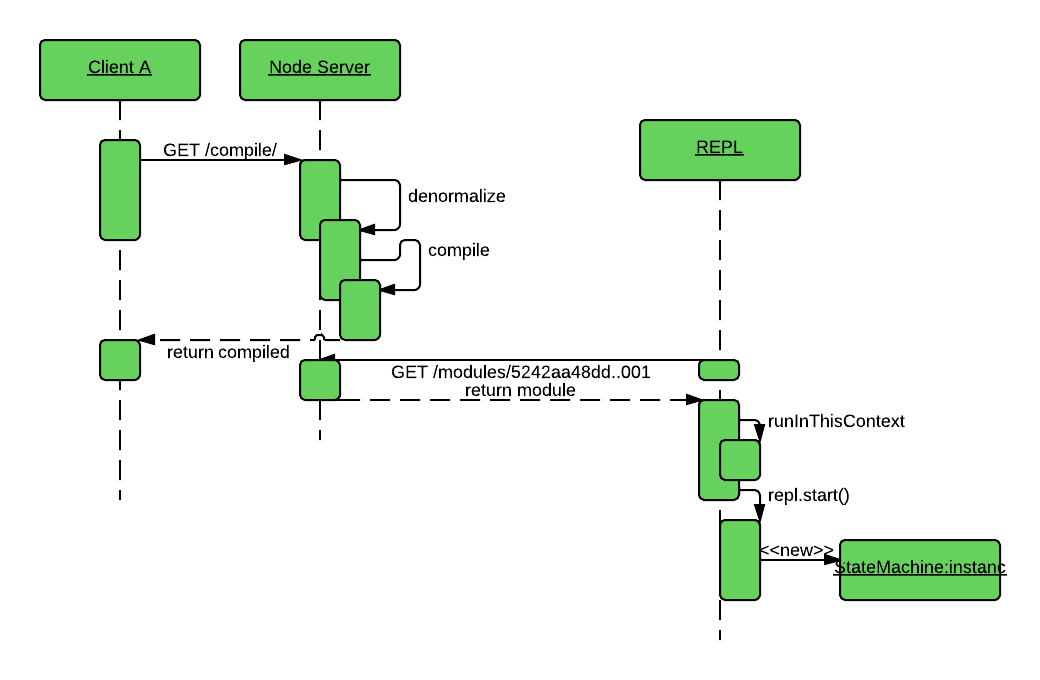
\includegraphics[width=15cm,keepaspectratio]{figures/compile-seq.png}
\caption{Kódgenerálás}
\label{fig:compileseq}
\end{figure}

A kollaboratív gráfszerkesztésen túl az alkalmazás egyszerű vizuális programozási nyelvek létrehozására alkalmas.
A vizuális programozás menete a következő egy minta nyelv példányán amiben állapotgépeket lehet programozni:
\begin{enumerate}
\item A kliensoldalon a felhasználó elkészíti a gráftranszformációs template kódot,
\item A felhasználó elkészíti egy vizuális implementációját a nyelvnek, vagyis egy konkrét állapot gépet vizuálisan,
\item A fordítás gomb megnyomása után a szerveralkalmazás denormalizálja a gráfot, azaz létrehoz egy olyan struktúrát, ami a diagramot reprezentálja redundánsan. Ez a struktúra a bemenő adata a gráftranszformáló template-nek,
\item A szerveralkalmazás a template alapján egy konkrét állapotátmenetekkel rendelkező állapotgép Javascript kódját hozza létre,
\item Ezt a kódot elmenti az adatbázisba és választ küld a kliensalkalmazásnak, ekkor kétféleképpen lehet felhasználni a kódot:
\begin{enumerate}
    \item A felhasználó böngészőjének Javascript parancssorában (példáúl Chrome Developer Console) értelmezi a kódot \lstinline{eval} segítségével és példányosítja az állapotgépet. 
    \item Node.JS parancssorból a mintrepl segédalkalmazással betölti a kódot, majd példányosítja az állapotgépet.
\end{enumerate}
\end{enumerate}


\subsubsection{Denormalizálás}

Az eredeti ``séma'' csúcsok listáját és élek listáját jelenti, viszont ez az adatformátum nem hasznos relációk kezelésére. Ezért reláció helyett redundancia bevezetésével oldom meg: egy diagram ilyen reprezentációjában egy él többször is jelenik meg. Ez leegyszerűsítve így néz ki:

\begin{lstlisting}[caption=Denormalizált -- vagy redundáns -- séma]
    {   edges: [
            {from: a, to: b},
            {from: a, to: c}],
        points: [
            {name: a, outgoing: [{from: a, to: b},{from: a, to: c}], incoming: []},
            {name: b, outgoing: [], incoming: [{from: a, to: b}]},
            {name: c, outgoing: [], incoming: [{from: a, to: c}]},
        ]
    }
\end{lstlisting}

Így ezen a struktúrán kevesebb kóddal írható egy olyan transzformáció ami valamilyen logikát valósít meg abból kiindulva, hogy milyen állapotból milyen élek mennek ki és be. Ez struktúra ami ilyenkor létrejön csak átmenetileg van felhasználva amíg kódot generál a szerveroldal, utána nem lesz használva semmire, így nem kella redundancia által okozott szokásos próblémákkal küzdeni. Ebben a formában tárolni mindig a gráfot nem hatékony, mert minden diagram manipulációs művelet több mint egy adatbázis lekérdezést jelentene és ha el szeretném kerülni a redundancia anomáliákat 
akkor megnövekedne fölöslegesen a komplexitás (tranzakciókra lenne szükség, vagy zárolásra és ezeket nem biztosítja a MongoDB). Ez a denormalizálás viszont csak két for ciklusból áll és ritkán fut le. 

\subsubsection{Gráftranszformáció template}

A gráftranszformáció template egy Underscore template. Underscore.JS egy Javascript könyvtár ami funkcionális programozás eszközökkel bővíti e nyelvet, anélkül, hogy kiterjesztené a beépített típusokat. \cite{underscorejs.org}
Ezen belül a template rendszer lehetővé teszi egy template fájlt lefordítását adott kontextus alapján. A template-ben \lstinline{<\%= \%>} segítségével változó behelyettesítés történik, \lstinline{<\% \%>} segítségével Javascript kódot lehet értelmeztetni. 

\begin{lstlisting}[caption=Underscore template lefordítása]
var compiled = _.template("hello: <%= name %>");
compiled({name: 'moe'});
=> "hello: moe"
\end{lstlisting}

Az alkalmazásban így néz ki felhasználói szemszögből:

\begin{figure}[!ht]
\centering
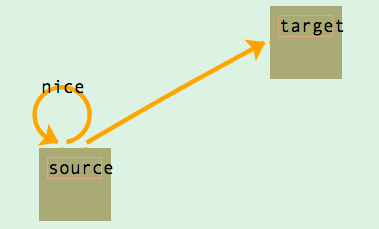
\includegraphics[width=5cm,keepaspectratio]{figures/simple-graph.png}
\caption{Egy példa diagram}
\label{fig:compileseq}
\end{figure}

\begin{lstlisting}[caption=A gráftranszformációs Underscore template]
Elements: 
<% 
    doc.entities.forEach(function(el){
%>
    <%= el.title %>
<%
    })
%>
\end{lstlisting}


\begin{lstlisting}[language=HTML,caption=Az eredmény]
Elements: 

source
target
\end{lstlisting}

Természetesen nem csak Javascript kódot lehet generáltatni az alkalmazásban, hiszen a template behelyettesítés eredménye egyszerű szöveg. 

Az állapotgép nyelvhez tartozó template , egy példa állapotdiagram és a generált kód megtekinthető a második függelékben.




%---------------------------------------------------
\subsubsection{A generált kód felhasználása}
%---------------------------------------------------

A generált kód elmentődik az adatbázisba a diagram egyik attribútumába, és ehhez az adathoz egy API végponton keresztül lehet hozzáférni és felhasználni meg akár a triviális HTML script elem segítségével:

\begin{lstlisting}[language=HTML]
 <script type="text/javascript" src="http://localhost:3000/api/compile/modules/5242aa48ddda9b0000000001/"></script>
\end{lstlisting}

Parancssorból is fel lehet használni \lstinline{node mintrepl <id>} segítségével, a mintrepl egy javascript szkript, ami a fent említett API-n keresztül letölti és értelmezi a fájlt, majd futtatja a letöltött kódot és egy REPL\footnote{Read-Eval-Print-Loop} interaktív node shell-t futtat. 

\begin{lstlisting}[caption=A generált kód felhasználása NodeJS shellben]
 $ node mintrepl 5242aa48ddda9b0000000001
 mint 5242aa48ddda9b0000000001> tanulo = new sm()
 mint 5242aa48ddda9b0000000001> tanulo.consumeEvent("kávé")
 mint 5242aa48ddda9b0000000001> tanulo.currentState
 ébren
 \end{lstlisting}

 Hasonló módon egy másik node szerver szerveroldali kódjába is be lehet illeszteni. 
 





